
\id{ҒТАМР 52.45.19}

\begin{articleheader}
	\sectionwithauthors{Г. Аскарова, Б.	Бектур, М.Шаутенов, А. Бегалинов}{АЛТЫНҚҰРАМДЫ КЕНДЕРДІҢ ГРАВИТАЦИЯЛЫҚ- ФЛОТАЦИЯЛЫҚ БАЙЫТУ ТЕХНОЛОГИЯСЫ}

{\bfseries \textsuperscript{1}Г. Аскарова, \textsuperscript{1,2}Б.
Бектур\textsuperscript{\envelope }, \textsuperscript{1}М.Шаутенов,
\textsuperscript{1}А. Бегалинов}
\end{articleheader}
\begin{affiliation}

\textsuperscript{1}Satbayev University, Тау-кен металлургиялық
институті, Алматы, Қазақстан,

\textsuperscript{2}АҚ «Майқаинзолото», Павлодар, Қазақстан

\raggedright{\bfseries \textsuperscript{\envelope }}Корреспондент-автор:\href{mailto:bekturbek@bk.run}{bekturbek@bk.ru}
\end{affiliation}

Бұл жұмыста құрамында алтыны бар Васильков кенорынның кенін
гравитациялық-флотациялық байытылымдығына байланысты зерттеулер
келтірілген. Технологиялық зерттеулерге сәйкес кендегі алтынның орташа
мөлшері 5,8 г/т ал күміс мөлшері шамамен -- 2,1 г/т. Сынамада негізгі
кен минералдары ретінде пирит пен арсенопирит сондай-ак пирротит
кездеседі. Бұл минералдардың кендегі орташа мөлшері минералогиялық және
рентгендік дифракциялық талдаулар бойынша шамамен 21.87\% (барлығы)
құрады. Бастапқы кенде негізгі таужыныс түзетін минералдар ретінде кварц
және кварц-хлорит-слюда агрегаттарынан (2.71\%), тұрады. Жүргізілген
зерттеу нәтижелері бойынша зерттеу кезінде алтынның шығымы 7,04\%,
концентраттың жалпы шығымы 21,57\% және құрамы 24,78 г/т екені
анықталды. Бұл ретте гравитациялық қалдықтағы алтынның мөлшері 2,4 г/т.
Кезеңдік зерттеу тек гравитациялық байыту технологиясын пайдалана
отырып, кенді өңдеу үшін үш сатылы байыту схемасын қолдану жөн екенін
көрсетті. Бірінші кезең -- 2,5 мм кен мөлшерінде ұсату 2 сатыда 0.4 мм
ге дейін ал 3 сатыда 0,2 мм үнтақтау жүргізілген.Байытудың 1-ші
кезенінде отсадкалау, концентрациялау столдарында және винттік бөлгіштер
қолданылады. Байытудың 2- 3 ші кезендерінде ұсақ алтынды бөліп алу
операциясы ретінде гидроцентрифугалық сепарация тиімді жұмыс істейді.
Осы байыту сұлбасы арқылы байыту фабрикасында 0.4 мм дейін ұсақталған
бірінші сатыдағы қалдықтарды байыту концентрат шығымдылығымен жалпы
гравитациялық концентратқа ұсақ және өте майда сап алтынды бөліп алу
мүмкіндігін берді. Бастапқы кенді гравитациялық және флотациялық байыту
нәтижелері біріктірілген гравитациялық-флотациялық технологиялық схеманы
қолданудың орындылығынкөрсетеді. Флотациялық байыту сұлбасы бойынша
бастапқы кенді байыту бойынша рН -8.0 кезінде келесі өнімдер алынды:
шығымы 14,53\% алтын мөлшері 13.3 г/т флотациялық концентрат (II қайта тазартудан кейін);
гравитациялық-флотациялық концентраттағы алтынның жалпы алынуы 21.57\%
шығымдылықпен және 20,87 г/т Au құрамымен флотациялық қалдықтардағы
алтынның мөлшері 0,72 г/т.

{\bfseries Түйін сөздер:} алтын, байытымдылығы, технологиялық зерттеулер,
флотация, гравитация, модельдеу, концентрат, қалдық, бөліп алу дәрежесі
\begin{articleheader}

{\bfseries ТЕХНОЛОГИЯ ГРАВИТАЦИОННО-ФЛОТАЦИОННОГО ОБОГАЩЕНИЯ
ЗОЛОТОСОДЕРЖАЩИХ РУД}

{\bfseries \textsuperscript{1}Г. Аскарова,
\textsuperscript{1,2}Б.Бектур\textsuperscript{\envelope },
\textsuperscript{1}М.Шаутенов, \textsuperscript{1}А. Бегалинов}
\end{articleheader}
\begin{affiliation}
\textsuperscript{1}Satbayev University, Горно-металлургический институт,
Алматы, Казахстан,

\textsuperscript{2}АО «Майкаинзолото», Павлодар, Казахстан,

e-mail: \href{mailto:bekturbek@bk.run}{bekturbek@bk.ru}
\end{affiliation}

В данной работе приведены исследования, связанные с
гравитационно-флотационным обогащением золотосодержащих руд
Васильковского месторождения. По данным технологических исследований,
среднее количество золота в руде составляет 5,8 г/т, а количество
серебра - около 2,1. г/т.Основными рудными минералами являются пирит,
арсенопирит и пирротин. Среднее содержание этих минералов в руде по
данным минералогического и рентгеноструктурного анализов составило около
21,87\% (суммарно). Первичная руда состоит из кварца и
кварц-хлорит-слюдяных агрегатов (2,71\%) как основных породообразующих
минералов.По результатам проведенных исследований установлено, что выход
золота за время исследований составил 7,04\%, общий выход концентрата -
21,57\%, состав - 24,78 г/т. При этом количество золота в гравитационном
остатке составляет 2,4 г/т. Поэтапное исследование показало, что для
переработки руды предпочтительно использовать трехстадийную схему
обогащения с применением только гравитационной технологии обогащения. На
первом этапе дробилось 2,5 мм руды, на 2-м этапе - 0,4 мм, на 3-м этапе
- 0,2 мм. На 1-й стадии обогащения используются отсадочные машины,
концентрационные столы и винтовые сепараторы.

Результаты гравитационно-флотационного обогащения первичной руды
показывают целесообразность использования комбинированной
гравитационно-флотационной технологической схемы. По схеме флотационного
обогащения от первичного обогащения руды при рН -8,0 были получены
следующие продукты: выход 14,53\%, содержание золота 13,3 г/т
флотоконцентрата (после II переочистки); общее извлечение золота в
гравитационно-флотационном концентрате с выходом 21,57\% и содержанием
Au 20,87 г/т, количество золота в хвостах флотации - 0,72 г/т.

{\bfseries Ключевые слова:} золото, обогащение, технологические
исследования, флотация, гравитация, моделирование, концентрат, хвосты,
извлечения.
\begin{articleheader}

{\bfseries TECHNOLOGY OF GRAVITY-FLOTATION ENRICHMENT OF GOLD ORES}

{\bfseries \textsuperscript{1}G. Askarova, \textsuperscript{1,2}B.
Bektur\textsuperscript{\envelope }, \textsuperscript{1}M. Shautenov,
\textsuperscript{1}А. Begalinov}
\end{articleheader}

\begin{affiliation}

\textsuperscript{1}Satbayev University, Mining and Metallurgical
Institute, Almaty, Kazakhstan,

\textsuperscript{2}JSC «Maykainzoloto», Pavlodar, Kazakhstan,

e-mail: \href{mailto:bekturbek@bk.run}{bekturbek@bk.ru}
\end{affiliation}

This paper presents studies related to gravity-flotation enrichment of
gold ores of the Vasilkovskoe deposit. According to technological
studies, the average amount of gold in the ore is 5.8 g/t, and the
amount of silver is about 2.1. g/t. The main ore minerals are pyrite,
arsenopyrite and pyrrhotite.The average content of these minerals in the
ore, according to mineralogical and X-ray diffraction analyses, was
about 21.87\% (total). The primary ore consists of quartz and
quartz-chlorite-mica aggregates (2.71\%) as the main rock-forming
minerals. Based on the results of the research, it was established that
the gold yield during the research was 7.04\%, the total concentrate
yield was 21.57\%, and the composition was 24.78 g/t. At the same time,
the amount of gold in the gravity residue is 2.4 g/t. A step-by-step
study showed that for ore processing it is preferable to use a
three-stage enrichment scheme using only gravity enrichment
technology.At the first stage, 2.5 mm of ore was crushed, at the 2nd
stage - 0.4 mm, at the 3rd stage - 0.2 mm. At the 1st stage of
enrichment, jigging machines, concentration tables and screw separators
are used.

The results of gravity-flotation enrichment of primary ore show the
feasibility of using a combined gravity-flotation technological scheme.
According to the flotation enrichment scheme, the following \\products
were obtained from the primary enrichment of ore at pH -8.0: yield
14.53\%, gold content 13.3 g/t of flotation concentrate (after II
repurification); total gold recovery in gravity-flotation concentrate
with a yield of 21.57\% and Au content of 20.87 g/t, the amount of gold
in the flotation tailings is 0.72 g/t;

Keywords: gold, beneficiation, technological research, flotation,
gravity, modeling, concentrate, tailings, extractions.
\begin{multicols}{2}

{\bfseries Кіріспе.} Заманауи ғылыми-зерттеу мен байыту технологияларының
үздіксіз дамуына, білім мен тәжірибе көлемі кеңейіп, аналитикалық және
басқа зерттегіш аспаптық базасының жетілуіне байланысты тау-кен өндіру
және байыту өнеркәсібі үздіксіз дамуда. Заманауи зерттеу жұмыстары
тау-кен өндірісі болғаннан бері жүргізіліп келеді. Қазақстанда, Ресей
Федерациясының аумағында да, Қытайдағы, Кореядағы, Бразилиядағы шетелдік
ғылыми зерттеу орталықтарында жүргізілген ғылыми жұмыстардың орасан зор
көлеміне қарамастан, оларды барынша кеннің құрамындағы пайдалы
компонентті барынша бөліп алу үшін көптеген зерттеулер жүргізілді.
Қазіргі таңда қиын байытылатын құрамында алтыны бар кендерден бағалы
компоненттері барынша бөліп алу барлық тау-кен, байыту және
металлургиялық кешендерді дамыту үшін өте өзекті мәселе болып табылады.
Зерттеудің мақсаты. Қиын байытылатын Васильков кенорнының кендерінің
және байыту өнімдерінің технологиялық қасиеттерін зерттеу негізінде
байытудың әдісі ретінде гравитациялық және флотациялық әдісін таңдау
және оны негіздеу, үрдістің негізгі көрсеткіштерін анықтау болып
табылады {[}1,2{]}.

Жұмыстың өзектілігі.Бұл технология қиын байытылатын алтын құрамды
кендерден құрамына асыл металдардан басқа барлық пайдалы компоненттерді
комплексті түрде бөліп алу технологиялық байыту сұлбасын құру
технологиялық тұрғыда ең маңыздыларының бірі деп санауға болады. Сондай
-ақ жасалған технологиялық байыту сұлбасы экономикалық және экологиялық
тұрғыда тиімді болуы керек. Сарапшылардың пікірінше қазіргі таңда
заманауи ХХІ ғасырда алтын құрамды қиын байытылатын және күрделі
кендерді пайдалануға кеңінен тарту арқылы әлемде алтын өндірудің негізгі
тиімді және экологиялық, экономикалық технологиясын жасақтау және осы
технологияны жетілдіруды қамтамасыз ету жоспарлануда.

Байыту фабрикаларының алдына қойылған мақсаттар мен міндеттерге жету
үшін, әдетте, әртүрлі күрделі өңдеу схемалары қолданылады:
гравитациялық-флотациялық, гравитациялық-металлургиялық және т.б.
Пайдалы минералды шикізатты байытудың белгілі бір байыту технологиясын
қолдану үшін әртүрлі факторларға байланысты -- бөлшектердің пішіні,
геометриялық өлшемдері, массасы, сулануы, минералдардардың бір бірімен
байланысы және т.б.

Сонымен қатар осы жұмыста өндірістік жағдайларда байыту
тиімділігінебайланысты бастапқы шикізат ірілігінің әсері туралы
зерттеулерді ұсынады. Жер қыртысындағы кездесетін алтынның химиялық
инерттілігіне байланысты барлығы дерлік алтын табиғатта сап алтын күйде,
атап айтқанда немесе басқада металл қоспаларымен кездеседі. Осы фактіні
және осы металдың физикалық қасиеттерін ескере отырып, минералдарды бөлу
үшін гравитациялық әдістерді қолдануға болады. Дегенмен, мұндай
технологияны ұсақ бөлінген шикізат болған жағдайда пайдалану көбінесе
құнды компоненттердің жоғары жоғалуымен және қоршаған ортаға теріс әсер
етеді {[}1{]}.

\emph{Зерттеу обьектісі.} Алтын құрамды Васильков кенорнының кендерінде
негізгі миенралдар ретінде келесі минералдар кездеседі: арсенопирит,
пирит, пиротит, марказит, алтын, халькопирит, сфалерит, галенит,
висмутин, молибденит, кубанит, борнит, тау-кен химиялық минералдары
ретінде: циркон, апатит, сфен, магнетит, ильменит, хромит, серицит,
хлорит, калишпат, турмалин), кварц, карбонаты (сидерит, анкерит,
кальцит), флюорит, барит. сппатит, ремагнетит, , ильменит, хромит,
серицит, хлорит, калий дала шпаты, турмалин), кварц, карбонаттар
(сидерит, анкерит, кальцит), флюорит, барит. Арсенопирит -- негізгі кен
минералы болып табылады. Кен 90\%кварцтан тұрады. ал сульфидтер 3-тен
5\%-ке дейін. Кенде сондай-ақ зиянды қоспа ретінде мышьяк бар оның үлесі
2\% тен жоғарыи более.~Кенді минералдар (сульфидтер) пирит -- 2,2\%,
арсенопирит -- белгілер түрінде көрсетілді; халькопирит пен галенитте
алтын сирек кездесетін. Бұл кен орнының кені құрамында сульфидті, ал
тотығу дәрежесі бойынша сульфидті болып келеді.Кеннің фазалық талдау
қорытындысы бойынша 1) кенді алдын-ала байыту қолданугға болады;2)-2,5
мм кеннің ірілігінде сап алтынның шығымы 30,12\% көрсетті. Кеннің
ірілігі кішірейген сайын --2,5 мм (--0,074мм)до65\%сап алтынның үлесі
өсе береді 52,50ден68,16\%көруге болады. 1-суретте Васильков кендегі
алтының әртүрлі фазалардағы микроқұрылымы келтірілген. Елеуішті талдау
арқылы кендегі алтының темірдің және күкірттің гранулометриялық
сипаттамасы 1-кесте көрсетілген.
\end{multicols}


\begin{figure}[H]
    \centering
    \begin{subfigure}[b]{0.32\textwidth}
        \centering
        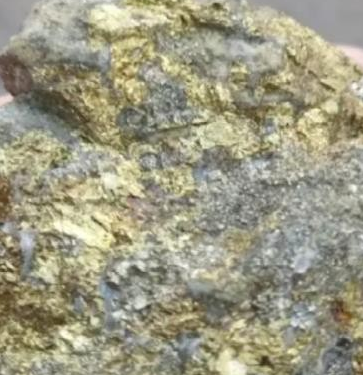
\includegraphics[width=\textwidth]{media/gor/image1}
        \caption*{a--алтынның пириттегі}
    \end{subfigure}
    \hfill
    \begin{subfigure}[b]{0.32\textwidth}
        \centering
        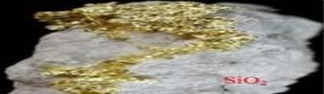
\includegraphics[width=\textwidth]{media/gor/image2}
        \caption*{ә--алтынның кварцпен}
    \end{subfigure}
    \hfill
    \begin{subfigure}[b]{0.32\textwidth}
        \centering
        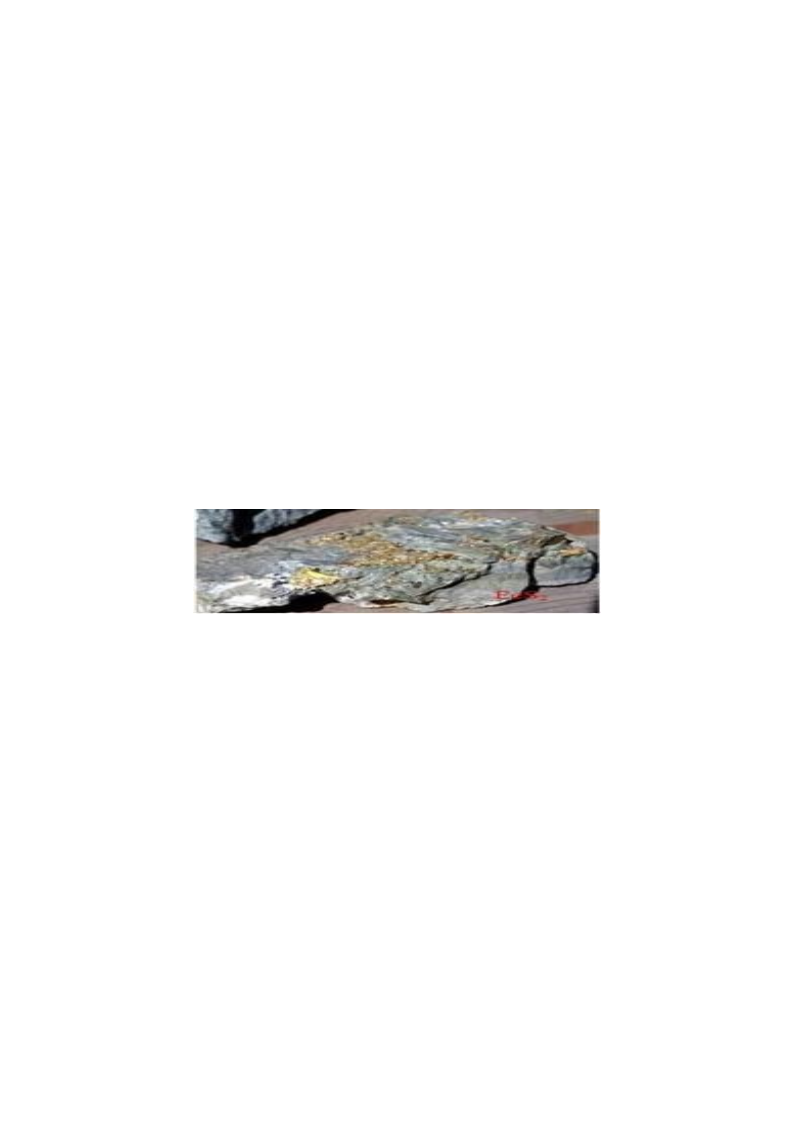
\includegraphics[width=\textwidth]{media/gor/image3}
        \caption*{б-алтынның пирит және арсенопиритпен}
    \end{subfigure}
    \caption*{1-сурет- Aлтынның әртүрлі фазалардағы микроқұрылымы}
\end{figure}



\begin{longtable}[H]{|@{}
  >{\raggedright\arraybackslash}p{(\columnwidth - 14\tabcolsep) * \real{0.1530}}|
  >{\raggedright\arraybackslash}p{(\columnwidth - 14\tabcolsep) * \real{0.1140}}|
  >{\raggedright\arraybackslash}p{(\columnwidth - 14\tabcolsep) * \real{0.1028}}|
  >{\raggedright\arraybackslash}p{(\columnwidth - 14\tabcolsep) * \real{0.0929}}|
  >{\raggedright\arraybackslash}p{(\columnwidth - 14\tabcolsep) * \real{0.1370}}|
  >{\raggedright\arraybackslash}p{(\columnwidth - 14\tabcolsep) * \real{0.1438}}|
  >{\raggedright\arraybackslash}p{(\columnwidth - 14\tabcolsep) * \real{0.1175}}|
  >{\raggedright\arraybackslash}p{(\columnwidth - 14\tabcolsep) * \real{0.1391}}|@{}}
\caption*{1-кесте. Кеннің - 2,5 мм ірілік класының гранулометриялық
сипаттамасы бойынша алтынның, темірдің, күкірттің таралуы {[}2{]}}\\
  \hline
\begin{minipage}[b]{\linewidth}\raggedright
  \textbf{Ірілік класы, мм}
\end{minipage} & \begin{minipage}[b]{\linewidth}\raggedright
  \textbf{Шығым, \%}
\end{minipage} & \begin{minipage}[b]{\linewidth}\raggedright
  \textbf{Алтынның үлесі, г/т}
\end{minipage} & \begin{minipage}[b]{\linewidth}\raggedright
  \textbf{Таралуы, \%}
\end{minipage} & \begin{minipage}[b]{\linewidth}\raggedright
  \textbf{Темірдің үлесі, \%}
\end{minipage} & \begin{minipage}[b]{\linewidth}\raggedright
  \textbf{Таралуы, \%}
\end{minipage} & \begin{minipage}[b]{\linewidth}\raggedright
  \textbf{Темірдің үлесі, \%}
\end{minipage} & \begin{minipage}[b]{\linewidth}\raggedright
  \textbf{Таралуы, \%}
\end{minipage} \\
\hline
+2,5 & 6.5 & 8.0 & 7,0 & 11,64 & 33,18 & 2,73 & 32,68 \\
\hline
-2,5+1.25 & 4.04 & 10.8 & 7.49 & 4,72 & 11,76 & 2,88 & 12,35 \\
\hline
-1.25+0.8 & 23.52 & 7.2 & 30.11 & 6,24 & 5,72 & 2,69 & 5,72 \\
\hline
-0.8+0.56 & 11.86 & 5.6 & 11.41 & 11,08 & 6,14 & 2,66 & 6,05 \\
\hline
-0.56+0.40 & 8.0 & 7.6 & 10.50 & 7,06 & 11,28 & 3,45 & 12,53 \\
\hline
-0.40+0.30 & 5.81 & 5.6 & 5.570 & 6,11 & 7,04 & 4,25 & 7,99 \\
\hline
-0.30+0.20 & 6.54 & 5.2 & 5.88 & 17,54 & 6,10 & 4,35 & 6,52 \\
\hline
-0.20+0.15 & 2.99 & 6.2 & 3.18 & 11,07 & 18,78 & 4,64 & 16,17 \\
\hline
-0.15+0.1 & 4.38 & 4 & 2.99 & 5,62 & 33,18 & 2,73 & 32,68 \\
\hline
-0.1+0.074 & 2.89 & 5.4 & 2.68 & 6,73 & 11,76 & 2,88 & 12,35 \\
\hline
-0.074 еленген & 3.78 & 4.8 & 3.14 & 5,77 & 5,72 & 2,79 & 5,72 \\
\hline
-0.074седим & 18.9 & 3.1 & 10.15 & 5,89 & 6,14 & 2,27 & 6,05 \\
\hline
Всего & 100 & 5.8 & 100 & 6.75 & 100 & 3.68 & 100 \\
\hline
\end{longtable}

% \begin{longtable}[H]{|@{}
%   >{\raggedright\arraybackslash}p{(\columnwidth - 14\tabcolsep) * \real{0.1530}}
%   >{\raggedright\arraybackslash}p{(\columnwidth - 14\tabcolsep) * \real{0.1140}}
%   >{\raggedright\arraybackslash}p{(\columnwidth - 14\tabcolsep) * \real{0.1028}}
%   >{\raggedright\arraybackslash}p{(\columnwidth - 14\tabcolsep) * \real{0.0929}}
%   >{\raggedright\arraybackslash}p{(\columnwidth - 14\tabcolsep) * \real{0.1370}}
%   >{\raggedright\arraybackslash}p{(\columnwidth - 14\tabcolsep) * \real{0.1438}}
%   >{\raggedright\arraybackslash}p{(\columnwidth - 14\tabcolsep) * \real{0.1175}}
%   >{\raggedright\arraybackslash}p{(\columnwidth - 14\tabcolsep) * \real{0.1391}}@{}|}
% \toprule\noalign{}
% \begin{minipage}[b]{\linewidth}\raggedright
% Ірілік класы, мм
% \end{minipage} & \begin{minipage}[b]{\linewidth}\raggedright
% Шығым, \%
% \end{minipage} & \begin{minipage}[b]{\linewidth}\raggedright
% Алтынның үлесі, г/т
% \end{minipage} & \begin{minipage}[b]{\linewidth}\raggedright
% Таралуы, \%
% \end{minipage} & \begin{minipage}[b]{\linewidth}\raggedright
% Темірдің үлесі, \%
% \end{minipage} & \begin{minipage}[b]{\linewidth}\raggedright
% Таралуы, \%
% \end{minipage} & \begin{minipage}[b]{\linewidth}\raggedright
% Темірдің үлесі, \%
% \end{minipage} & \begin{minipage}[b]{\linewidth}\raggedright
% Таралуы, \%
% \end{minipage} \\
% \midrule\noalign{}
% \endhead
% \bottomrule\noalign{}
% \endlastfoot
% +2,5 & 6.5 & 8.0 & 7,0 & 11,64 & 33,18 & 2,73 & 32,68 \\
% -2,5+1.25 & 4.04 & 10.8 & 7.49 & 4,72 & 11,76 & 2,88 & 12,35 \\
% -1.25+0.8 & 23.52 & 7.2 & 30.11 & 6,24 & 5,72 & 2,69 & 5,72 \\
% -0.8+0.56 & 11.86 & 5.6 & 11.41 & 11,08 & 6,14 & 2,66 & 6,05 \\
% -0.56+0.40 & 8.0 & 7.6 & 10.50 & 7,06 & 11,28 & 3,45 & 12,53 \\
% -0.40+0.30 & 5.81 & 5.6 & 5.570 & 6,11 & 7,04 & 4,25 & 7,99 \\
% -0.30+0.20 & 6.54 & 5.2 & 5.88 & 17,54 & 6,10 & 4,35 & 6,52 \\
% -0.20+0.15 & 2.99 & 6.2 & 3.18 & 11,07 & 18,78 & 4,64 & 16,17 \\
% -0.15+0.1 & 4.38 & 4 & 2.99 & 5,62 & 33,18 & 2,73 & 32,68 \\
% -0.1+0.074 & 2.89 & 5.4 & 2.68 & 6,73 & 11,76 & 2,88 & 12,35 \\
% -0.074 еленген & 3.78 & 4.8 & 3.14 & 5,77 & 5,72 & 2,79 & 5,72 \\
% -0.074седим & 18.9 & 3.1 & 10.15 & 5,89 & 6,14 & 2,27 & 6,05 \\
% Всего & 100 & 5.8 & 100 & 6.75 & 100 & 3.68 & 100 \\
% \end{longtable}
\begin{multicols}{2}

{\bfseries Материалдар мен әдістер.} Зерттеу объектісі болып алтынқұрамды
Васильков кен орнының сынамалары қолданылды.

Зерттеулерді жүргізу үшін кен сынамасын стандартты әдістер бойынша
алдымен ұсатып және орташа сынама алынды. Кен сынамасының массасы 12 кг
болды.

Кеннің элементтік, фазалық және минералогиялық құрамын анықтау үшін
келесідей физика-химиялық зерттеу әдістері қолданылды:
рентгенфлуоресценциялық, рентгендифракциялық, микроскопиялық және
химиялық. Рентгенфлуоресценциялық талдау әдісі SciAps Х-50 аппаратымен,
рентгендифракциялық талдау Pert MPDPRO (PANalytical) қондырғысымен,
микроскопиялық талдау - Axio Scope.A1 қондырғысымен жүргізілді.

Кен сынамасынның гранулометриялық құрамын анықтау үшін седиментациялық
талдау әдісімен анықталды. Седиментациялық талдауда сұйық орта ретінде
су алынды. Ұсатылған фракциялардағы алтын мен негізгі элементтердің
нақты құрамын білу үшін рационалды құрам есептелді, кен массасы 100 г
болды. Әр фракциядағы алтынның мөлшері химиялық талдаумен анықталды.
Кенді байыту гравитациялық әдіспен, 1-суреттегі сұлба бойынша жүргізілді
{[}2,3{]}.

Кеннің заттық құрамын зерттеу нәтижелері бойынша 65\% -0,074 мм бөлшек
мөлшеріне дейін ұсақталғанда алтынның жартысынан көбі (65,16\%) бос
күйінде болатынын көрсетті. Сондықтан бұл кенді өңдеу үшін гравитациялық
байыту әдістерін қолдану тиімді екеін көрсетіп, атап айтқанда,
отсадкалау машинасында, винтті бөлгіште және тазалау операциясы ретінде
концентрациялау столында байыту ал кендегі ұсақ алтын түйіршіктерін
(1,5\%-ға дейін) бөліп алу үшін гидроконцентрат қолданды шығымдылығымен
салыстырғанда басқа центрифугалық апппараттардан жоғары (1,5\%-дан
астам) болғанын көрсетті.Кен орнының кендегі бос сап алтынды бөліп алу
үшін орталықтан тепкіш әдістерді қолдану мүмкіндігі
анықталды.Гравитациялық әдістерді қолдана отырып, кеннің аралық
мөлшерінде (65\% -0,074 мм) бос алтын алу деңгейін кеңейтілген байыту
сынақтарының нәтижелері бойынша бағаланды. Концентрат шығымының алтынның
алынуына әсері концентратты үздіксіз түсіру арқылы отсадкалау
машинасындағы кен байытуды модельдеу нәтижелері бойынша анықталды. Жалпы
алғанда, кен орнындағы кенді гравитациялық әдістермен байыту бойынша
зерттеулердің сатысында келесі сынақтар жүргізілді:--- 1-ші сынағы оның
мақсаты ауырлық күшімен алынатын алтынның мөлшерін анықтау және ортадан
тепкіш күш арқылы бөлініп алынатын гидроконцентраторды қолдану
мүмкіндігін бағалау болды. 2-ші кен орнын байыту үшін концентрат шығымы
төмен сепараторлар жүргізу әдістемесі бойынша кенді үш сатылы байытуды
қолдану: бірінші кезеңде кеннің ірілігі -2,5 мм (1,9) мм, екіншіде --
шамамен -0,4 мм, үшіншіде -0,2 мм. Гравитация байытудың нәтижелері
2-кестеде берілген.

Тәжірибе ортадан тепкіш гидроконцентраторларда байыту жүргізілді, әрбір
сатыда сол сатыға сай кен ірілігі дәйекті түрде азайтылып отырды.
Бастапқы кеннің ірілігі --2,5 ммден -- 0,074 мм 26,99-65\% ірілік
аралығында зерттелді. Әр кезеңде 4 байыту операциясы орындалды (бірінші
кезеңде -- 2 операция).

Зерттеу объектісі болып алтынқұрамды Васильков кен орнының сынамалары
табылды. Зерттеулерді жүргізу үшін кен үлгілері стандартты әдістер
бойынша алдымен ұсақталды және орташа сынама алынды. Кен сынамасының
массасы 12 кг болды.Кеннің элементтік, фазалық және минералогиялық
құрамын анықтау үшін келесідей физика-химиялық зерттеу әдістері
қолданылды: рентгенфлуоресценциялық, рентгендифракциялық, микроскопиялық
және химиялық. Рентгенфлуоресценциялық талдау әдісі SciAps Х-50
аппаратымен, рентгендифракциялық талдау Pert MPDPRO (PANalytical)
қондырғысымен, микроскопиялық талдау - Axio Scope.A1 қондырғысымен
жүргізілді.Кен үлгілерінің гранулометриялық құрамы седиментациялық
талдау әдісімен анықталды. Седиментациялық талдауда сұйық орта ретінде
су алынды. Ұсақталған фракциялардағы алтын мен негізгі элементтердің
нақты құрамын білу үшін рационалды құрам есептелді, кен массасы 100 г
болды. Әр фракциядағы алтынның мөлшері химиялық талдаумен анықталды.
Кенді байыту гравитациялық әдіспен, 1-суреттегі сұлба бойынша
жүргізілді.

Нәтижелер мен талқылау

Қиын байытылатын алтынқұрамды кеннен алтынды толығымен бөліп алу әдісін
таңдау үшін алдымен кеннің сапалық және сандық талдауларының мәні
негізгі көрсеткіштер болып табылады. Зерттеуде алдымен
рентгенфлуоресценциялық және химиялық талдаулар көмегімен алдымен
Васильков алтынқұрамды кеннің химиялық құрамы анықталды (2-кесте).
\end{multicols}


\begin{longtable}{|>{\raggedright\arraybackslash}p{0.05\textwidth}|%
  >{\raggedright\arraybackslash}p{0.25\textwidth}|%
  >{\raggedright\arraybackslash}p{0.40\textwidth}|%
  >{\raggedright\arraybackslash}p{0.20\textwidth}|}
  \caption*{2 -- кесте Васильков алтынқұрамды кеннің химиялық құрамы}\\
  \hline
  \textbf{№} & \textbf{Элемент, қосылыс атауы} & \textbf{Химиялық формуласы, символы} & \textbf{Бағалы заттың үлесі, \%} \\
  \hline
  \endfirsthead
  
  \hline
  \textbf{№} & \textbf{Элемент, қосылыс атауы} & \textbf{Химиялық формуласы, символы} & \textbf{Бағалы заттың үлесі, \%} \\
  \hline
  \endhead
  
  \hline
  \endfoot
  
  \hline
  \endlastfoot
  
  \hspace{0.2cm} 1 & Кремний оксиді & SiO\textsubscript{2} & 64,62 \\
  \hline
  \hspace{0.2cm} 2 & Алюминий оксиді & Al\textsubscript{2}O\textsubscript{3} & 12,40 \\
  \hline
  \hspace{0.2cm} 3 & Кальций оксиді & CaO & 4,20 \\
  \hline
  \hspace{0.2cm} 4 & Магний оксиді & MgO & 3,43 \\
  \hline
  \hspace{0.2cm} 5 & Темір жалпы & Fe\textsubscript{жал} & 4,70 \\
  \hline
  \hspace{0.2cm} 6 & Күкірт жалпы & S\textsubscript{жал} & 1,22 \\
  \hline
  \hspace{0.2cm} 7 & Сульфидті күкірт & S\textsubscript{сульфид} & 1,18 \\
  \hline
  \hspace{0.2cm} 8 & Титан оксиді & TiO\textsubscript{2} & 0,43 \\
  \hline
  \hspace{0.2cm} 9 & Мыс & Cu & 0,24 \\
  \hline
  \hspace{0.2cm} 10 & Қорғасын & Pb & 0,05 \\
  \hline
  \hspace{0.2cm} 11 & Мырыш & Zn & 0,01 \\
  \hline
  \hspace{0.2cm} 12 & Мышьяк & As & 2,22 \\
  \hline
  \hspace{0.2cm} 13 & Алтын, г/т & Au & 3,20 \\
  \hline
  \hspace{0.2cm} 14 & Күміс г/т & Ag & 2,10 \\
 
  
  \end{longtable}
  

\begin{multicols}{2}

Рентгендифракциялық талдау нәтижесінде кеннің негізгі минералдары болып
арсенопирит, пирит, пирротин, өте аз мөлшерде халькопирит, сфалерит,
галенит, сфалерит, висмутин және т.б. бар екендігі табылды.
Минералогиялық талдау бойынша Васильков кеноры үлгісінде сап алтын,
сонымен қатар пирит, арсенопирит, аз мөлшерде халькопирит және висмутин,
сондай-ақ мышьякпен бірге байланысқан түрде кездесетіндігі анықталды.
Алтынның негзгі массасы ұсақдисперсті, пішіндері дұрыс емес, алтын
бөлшектерінің беті бос минералдармен жабылған.Мұндай «алтынтасушы»
минералдардың болуы кеннің қиын байытылатын түріне жататындығын
анықтайтын факторлар болып табылады {[}5, 6{]}.

Алтынқұрамды кеннің химиялық талдауы көрсеткендей, сынамалардағы
алтынның мөлшері оншалықты жоғары емес, небары 3,2 г/т тең болды.
Сынаманың басым көп бөлігі кварц болып табылды және оның мөлшері
64,62\%, ал алюминий оксидінің мөлшері шамамен 12.40 \% құрады.
Минерологиялық талдауға сәйкес алтынқұрамды кен сульфидті минералданған,
орташа гранодиориттер құрамды болып табылды{[}5,6{]}. Кен
сынамаларындағы алтынның кендегі кездесетін мөлшерін дәл анықтау үшін
рационалды құрам есептелді. Нәтижелер 3-кестеде келтірілген.
\end{multicols}


\begin{longtable}[H]{|@{}
  >{\raggedright\arraybackslash}p{(\columnwidth - 6\tabcolsep) * \real{0.0558}}|
  >{\raggedright\arraybackslash}p{(\columnwidth - 6\tabcolsep) * \real{0.4834}}|
  >{\raggedright\arraybackslash}p{(\columnwidth - 6\tabcolsep) * \real{0.2329}}|
  >{\raggedright\arraybackslash}p{(\columnwidth - 6\tabcolsep) * \real{0.2280}}|@{}}
  \caption*{3--кесте. Кендегі алтынның рационалды құрамы}\\

\hline
\hspace{0.2cm}\textbf{№} & \textbf{Алтынның минералдармен бірлесу нысаны} & \textbf{Бағалы заттың үлесі, г/т} & \textbf{Таралуы, \% }\\
\hline
\endhead
\hline
\endlastfoot
\hspace{0.2cm}1 & Сап алтын & 1,81 & 68,75 \\
\hline
\hspace{0.2cm}2 & Сульфидтер (арсенопиритпен) бірге & 2,11 & 21,87 \\
\hline
\hspace{0.2cm}3 & Сульфидтермен (пиритпен) байланысқан түрі & 0,64 & 6,67 \\
\hline
\hspace{0.2cm}4 & Тау жыныстарымен (кварц, доломит және т.б.) байланысқан түрі & 0,26 & 2,71 \\
\hline
& Барлығы & 3,20 & 100 \\

\end{longtable}

\begin{multicols}{2}

Кенді рационалды талдау нәтижесі бойынша алтынның басым бөлігі, яғни
68,75 \% мөлшері бос күйінде (1,8 г/т), шамамен бестен бір бөлігі
арсенопиритпен, 21.87\% - 2,1 г/т, он бестен бір бөлігі пиритпен (6,67
\%, 0,64 г/т) ал қалғаны - тау жыныстары минералдарымен (2,71 \% - 0,26
г/т) байланысқан түрде кездесетіндігі анықталды.

Ұсатылған кен сынамаларындағы алтынның әр ірілік класындағы таралу
мөлшерін анықтау үшін химиялық (дисперсті) талдау жүргізілді. Нәтижелер
4-кестеде келтірілген{[}4{]}.
\end{multicols}


\begin{longtable}[H]{|@{}
  >{\raggedright\arraybackslash}p{(\columnwidth - 6\tabcolsep) * \real{0.2429}}|
  >{\raggedright\arraybackslash}p{(\columnwidth - 6\tabcolsep) * \real{0.2443}}|
  >{\raggedright\arraybackslash}p{(\columnwidth - 6\tabcolsep) * \real{0.2458}}|
  >{\raggedright\arraybackslash}p{(\columnwidth - 6\tabcolsep) * \real{0.2670}}|@{}}
  \caption*{4 -- кесте. Әр түрлі класс бойынша алтынның дисперстік талдауы}\\
  
\hline
\textbf{Классы, мкм} & \textbf{Шығым,\%} & \textbf{Алтының, бағалы заттың құрамы, г/т} & \textbf{Таралуы,\% }\\
\hline
\endhead
\hline
\endlastfoot
+60 & 24,63 & 1,80 & 41,70 \\
\hline
-60+40 & 19,18 & 1,10 & 19,85 \\
\hline
-40+20 & 18,60 & 0,065 & 11,37 \\
\hline
-20+0 & 37,59 & 0,50 & 27,08 \\
\hline
Барлығы & 100,00 & 3,20 & 100,0 \\

\end{longtable}



\begin{figure}[H]
	\centering
	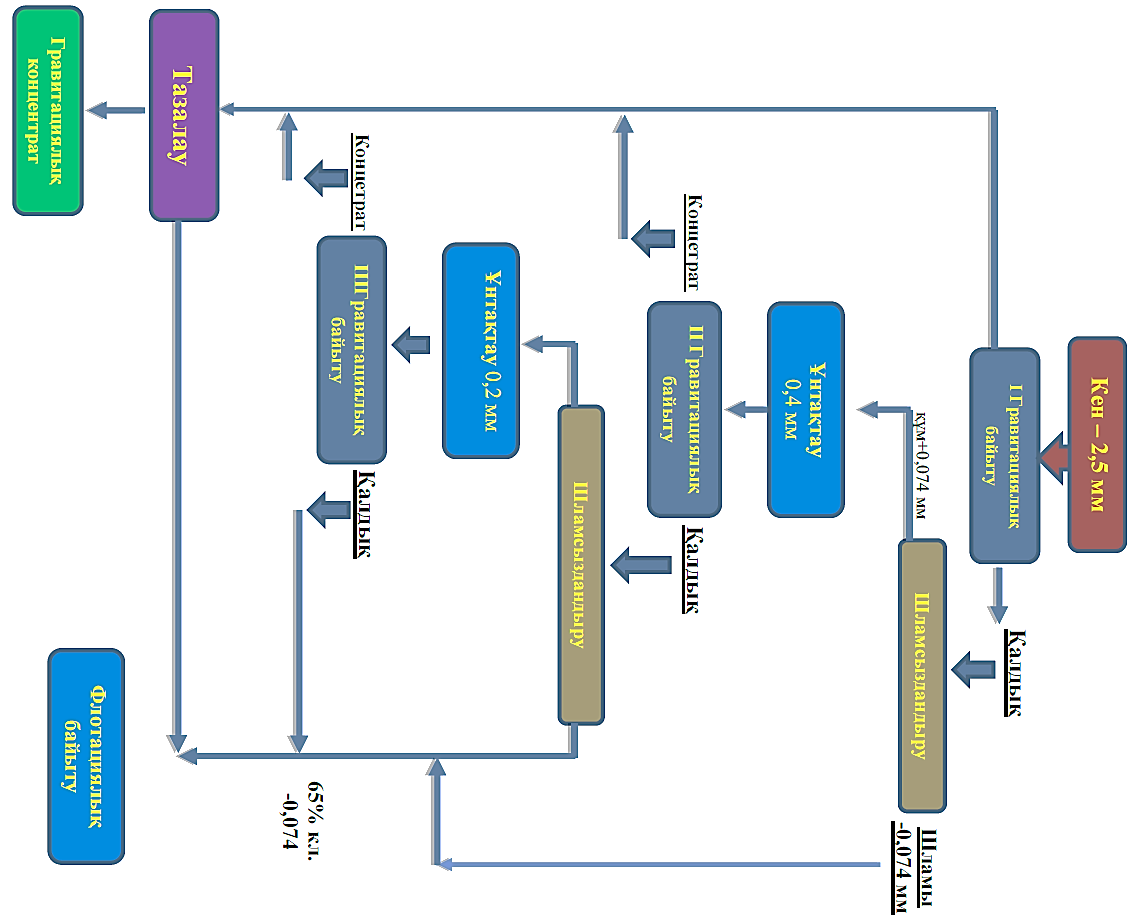
\includegraphics[width=0.6\textwidth]{media/gor/image4}
	\caption*{2 -- сурет. Aлтынқұрамды кеннің гравитациялық байыту сұлбасы}
\end{figure}


\begin{longtable}[H]{|@{}
  >{\raggedright\arraybackslash}p{(\columnwidth - 6\tabcolsep) * \real{0.2499}}|
  >{\raggedright\arraybackslash}p{(\columnwidth - 6\tabcolsep) * \real{0.2498}}|
  >{\raggedright\arraybackslash}p{(\columnwidth - 6\tabcolsep) * \real{0.2498}}|
  >{\raggedright\arraybackslash}p{(\columnwidth - 6\tabcolsep) * \real{0.2506}}|@{}}
  \caption*{5--кесте. Васильков алтынқұрамды кенді үш сатылы гравитациялық
  байыту нәтижелері}\\
\hline
\textbf{Өнімнің аттары} & \textbf{Шығымы, \%} & \textbf{Бағалы заттың пайыздық үлесі г/т} & \textbf{Бөліп алу дәрежесі,\%} \\
\hline
1 ші гравитациялық концентрат & 2,11 & 22,1 & 14.57 \\
\hline
Қалдық & 97,89 & 2,39 & 85.43 \\
\hline
2 ші гравитациялық концентрат & 2,86 & 20,5 & 18,32 \\
\hline
Қалдық & 97,14 & 2,0 & 81.68 \\
\hline
3-ші гравитациялық концентрат & 2,07 & 25,2 & 16.3 \\
\hline
Қалдық & 97,93 & 2,4 & 83.7 \\
\hline
Кен & 100 & 3,2 & 100 \\
\hline
\end{longtable}

% \begin{longtable}[H]{@{}
%   >{\raggedright\arraybackslash}p{(\columnwidth - 6\tabcolsep) * \real{0.2499}}
%   >{\raggedright\arraybackslash}p{(\columnwidth - 6\tabcolsep) * \real{0.2498}}
%   >{\raggedright\arraybackslash}p{(\columnwidth - 6\tabcolsep) * \real{0.2498}}
%   >{\raggedright\arraybackslash}p{(\columnwidth - 6\tabcolsep) * \real{0.2506}}@{}}
% \toprule\noalign{}
% \endhead
% \bottomrule\noalign{}
% \endlastfoot
% Өнімнің аттары & Шығымы, \% & Бағалы заттың пайыздық үлесі г/т & Бөліп
% алу дәрежесі,\% \\
% 1 ші гравитациялық концентрат & 2,11 & 22,1 & 14.57 \\
% Қалдық & 97,89 & 2,39 & 85.43 \\
% 2 ші гравитациялық концентрат & 2,86 & 20,5 & 18,32 \\
% Қалдық & 97,14 & 2,0 & 81.68 \\
% 3-ші гравитациялық концуентрат & 2,07 & 25,2 & 16.3 \\
% Қалдық & 97,93 & 2,4 & 83.7 \\
% Кен & 100 & 3,2 & 100 \\
% \end{longtable}
\begin{multicols}{2}

Зерттеулер нәтижесінде гравитациялық байыту әдісінің онтайлы байыту
сұлбасы алынды 2-суретте келтірілген.

Зерттеулердің барысында Васильков алтынқұрамды кенін байытудың тиімді
технологиялық сұлбасы құрастырылды, алынған көрсеткіштер бойынша
флотацияға жіберілетін қалдықта небары 2,4 г/т сап алтын бар, бұл
бұрынғы байыту сұлбасымен салыстырғанда әлдеқайда төмен болды, демек
барлық концентраттың шығымы 7.04\%, ал алтынды бөліп алу дәрежесі 49.19
\% көрсетеді. Бұл көрсеткіш дәстүрлі әдістермен алтынқұрамды кенді
байыту көрсеткіштерінен 1,5 есеге көп екенін келтірілген. Кенді
флотациялық байытудың технологиялық сынамасын зерттеу бастапқы кен және
гравитациялық байыту әдісінің қалдықтарында жүргізілді.

Құрамында сульфидті алтын бар концентратты алу үшін оңтайлы флотация
режимін әзірлеу мақсаты қойылды: кенді ұнтақтау мөлшері, реагент режимі,
пульпа тығыздығы, флотация уақыты т.б. факторларды қолданып флотациялық
байыту әдісін модельдеу арқылы оңтайлы технологиялық байыту сұлбасы
табылды. Бастапқы кеннің ұнтақтаудың оңтайлы өлшемін анықтау үшін
флотация үшін бастапқы кенді ұнтақтаудың оңтайлы ірілігін анықтау үшін
бөлшектердің мөлшері --0,074 мм (70--95\%) сынамаға бірқатар сынақтар
жүргізілді ұнтақтау кинетикасы табылды. Зерттеудің бастапқы кезеңінде
көбіктендіргіш ретінде С7 пайдаланылды жинағыш ретінде бутилді
ксантогенат қолданылды. Флотация байыту әдісінде ортаның 08,04 табиғи
деңгейінде жүргізілді. Негізгі, бақылау және тазалау флотациялық
операциялары жүргізілді.Әрбір тәжірибедегі флотациялық байыту әдісінің
нәтижелерін бағалау үшін флотация процесінің тиімділігін сипаттайтын
Хенкок критерийінің мәні есептелді.

Флотация кинетикасын зерттеу үшін көбіктендіргіш реагенттінің түрі мен
онтайлы шығынын таңдау үшін кенді әртүрлі ірілікте ұнтақтап алып
флотация жүргізілді. Көбіктендіргіш реагенттінің бірнеше түрі (қарағай
майы, Т-66 және Т-80 , С7 ) қолданылып сонын ішінде С7көбіктендіргіш
ретінде реагентті ретінде пайдаланылды. Жыйнағыш реагенттің шығымын,
флотация уақыты және оңтайлы ірілікті математикалық модельдеу арқылы
табылды.

Ұсынылған технологиялық сұлба бойынша талдау нәтижелері төмендегі
5-кестеде келтірілген.

Математикалық модельдеу арқылы флотациялық байыту әдісінің режимі:

-кенді ұнтақтау ірілігі 1-ші сатыда-75\% класса-0.074 мм;

-кенді ұнтақтау ірілігі 1-ші сатыда-85\% класса-0.074 мм;

- бутилдіксантогенаттың шығыны-150г/т;

-с-7 көбіктендіргіштің шығыны-70 г/т;

-мыс купоросының шығыны- 150 г/т;

-ортаны реттегіш реагентінің соданың шығыны-125 г/т;

-І негізгі флотацияның уақыты-15 мин;

-ІІ негізгі флотацияның уақыты-10 мин;

-ІІІ негізгі флотацияның уақыты-15 мин;

Васильков кенішінің алтын құрамды кенін математикалық модельдеу және
зерттеулер арқылы флотациялық онтайлы байыту сұлбасы алынды 3- суретте
келтірілген.
\end{multicols}

\begin{figure}[H]
	\centering
	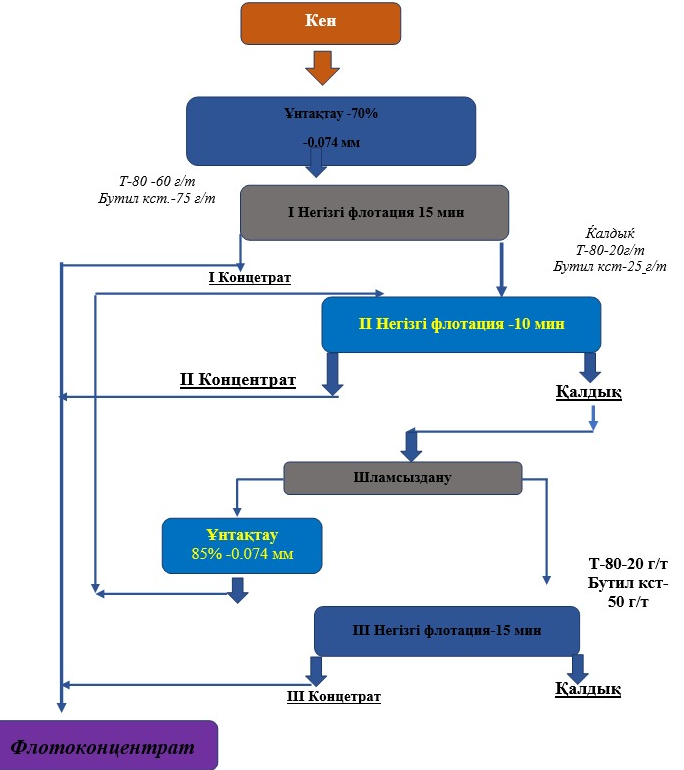
\includegraphics[width=0.8\textwidth]{media/gor/image5}
	\caption*{3-сурет. Aлтын құрамды кеннің флотациялық байыту сұлбасы}
\end{figure}


\begin{multicols}{2}

Көбікті концентратының шығыны, көбікті қабатының түрі эксперименталды
түрде таңдалды. Қолданылатын флотациялық байыту процестерінің
технологиялық тиімділігін бағалау үшін Луйкен-Хенкок формуласы
қолданылды:

\(E = \frac{\gamma(\beta - \alpha)}{\alpha(1 - \alpha)}\),

мұндағы α -- бастапқы кендегі бағалы заттың пайыздық үлесі; β -
байытылған өнімдегі бағалы заттың пайыздық үлесі; γ - байытылған өнімнің
шығымы.

Процесс E \textgreater{} 75\% болғанда өте тиімді, E \textgreater{} 50\%
болса тиімді, E \textless{} 25\% болғанда тиімсіз болып саналады.

Алтын құрамды қиын байытылатын Васильковка кенорнының гравитациялық және
флотациялық байыту әдстерін қолданылған технология бойынша байыту
нәтижесі төмендегі кестеде келтірілген {[}8{]}.
\end{multicols}

\begin{longtable}[]{|@{}
  >{\raggedright\arraybackslash}p{(\columnwidth - 6\tabcolsep) * \real{0.2273}}|
  >{\raggedright\arraybackslash}p{(\columnwidth - 6\tabcolsep) * \real{0.1515}}|
  >{\raggedright\arraybackslash}p{(\columnwidth - 6\tabcolsep) * \real{0.3636}}|
  >{\raggedright\arraybackslash}p{(\columnwidth - 6\tabcolsep) * \real{0.2576}}|@{}}
  \caption*{6 --кесте. Алтын құрамды қиын байытылатын Васильковск кенорнының
  гравитациялық және флотациялық байыту әдстерін қолданылған технология
  бойынша байыту нәтижесі}\\

\hline
\begin{minipage}[b]{\linewidth}\raggedright
  \textbf{Өнімдердің аты}
\end{minipage} & \begin{minipage}[b]{\linewidth}\raggedright
  \textbf{Шығымы, \%}
\end{minipage} & \begin{minipage}[b]{\linewidth}\raggedright
  \textbf{Бағалы заттың пайыздық үлесі, г/т}
\end{minipage} & \begin{minipage}[b]{\linewidth}\raggedright
  \textbf{Бөліп алу дәрежесі, \%}
\end{minipage} \\
\hline
Гравитациялық концентрат & 7.04 & 20.2 & 49.19 \\
\hline
Флотоконцентрат & 14.53 & 13.3 & 43.88 \\
\hline
Флотацияқалдығы & 78.43 & 0.42 & 6.93 \\
\hline
Кен & 100 & 3.2 & 100 \\
\hline
\end{longtable}
\begin{multicols}{2}

Тәжірибенің нәтижелері қиын байытылатын алтын құрамды кеннен флотациялық
қалдықтарды алуға болатынын көрсетеді. Ол үшін кенді ұнтақтау мөлшері
кемінде 85\% -0.074 мм класты сатылы флотациялық байыту сұлбасын қажет
екенін көрсетеді. 0,05 мм-ден аз. тазалау операцияларын қолдану
керектігін көрсетеді, флотациялық концентраттың шығымы 13,3 г/т алтынмен
14,53\% құрады. Бұл жағдайда жалпы қалдықтың шығымы 78,43\% бұндағы
алтынның мөлшері 0,42 г/т флотациялық қалдық алынды. гравитациялық және
флотациялық концентраттардың жалпы шығымы 21.57\% алтынның орташа
мөлшері г/т болғанда 16.8 құрады.

{\bfseries Қорытынды.} Қазіргі таңда отандық және шетелдік кәсіпорындардың
байыту фабрикаларының қолданылып отырған қиын байытылатын және баланстан
тыс кендерді байытудың біріктірілген гравитациялық және флотациялық
технологиялары кенді дайындаудың және байытудың заманауи сұлбаларын
сондай-ақ реагенттердің кең спектрін пайдалана отырып байыту
технологиясы әзірленді.

Технологиялар қолда бар реагенттер мен алтын құрамды қиын байытылатын
кендерды, қарапайым және ұтымды техникалық шешімдерді пайдалана отырып,
кендегі барлық пайдалы компоненттерді комплексті түрде бөліп алудың
нақты деңгейін негіздей отырып, кенненнемесе бастапқы шикізаттан сапалы
тауарлық өнім алуға мүмкіндік берді.

Технологиялар мүмкіндік береді:

1)Қиын байытылатын алтынқұрамды кеннен алтын және басқа пайдалы
компонентті комплескті түрде бөліп алуға;

2)жаңа кен орындарын игеруге ондағы бағалы металдар өндірісінің көлемін
ұлғайту;

3) қолайлы экологиялық жағдайды қалпына келтіру.

Бастапқы алтынқұрамды қиын байытылатын Васильковск кенорнының кеніне
гравитациялық және флотациялық байыту нәтижелері біріктірілген
гравитациялық-флотациялық технологиялық сұлбаны қолданудың орындылығын
көрсетеді.

Флотациялық ортаның рН мәнінде (қышқыл қоспай) гравитациялық-флотациялық
сұлбаны қолдана отырып, бастапқы кенді байытуда тәжірибесінде келесі
өнімдер алынды: гравитациялық концентраттың шығым 7.04\% ондағы алтынның
мөлшері 20.2 г/т флотациялық концентраттың шығымы 14.53\% алтынның
мөлшері 13.3 г/т және қалдықтың шығымғы 78.43\% және алтын мөлшері 0.42
г/т.

Алғыс. Мақала 2024-2026 жылдарға арналған гранттық қаржыландыру
шеңберінде АР23488914 «Табиғи және техногендік объектілердегі жұқа
дисперсті алтынды сандық бағалау технологиясын әзірлеу және оны
Қазақстан аумағында табу перспективаларын бағалау» жобасы бойынша
ғылыми-зерттеу жұмыстарының нәтижелері бойынша жазылған, жоба жетекшісі,
т.ғ.к., профессор М.Р.Шаутенов. Жоба тақырыбы бойынша зерттеулер
Қазақстан Республикасы ғылым және жоғары білім министрлігінің Ғылым
комитетімен қаржыландырылған.
\end{multicols}

\begin{center}
	{\bfseries Әдебиеттер}
	\end{center}
	
	\begin{references}

1. Федотов П. К., Сенченко А. Е., Федотов К. В., Бурдонов А. Е..
Исследование обогатимости убогосульфидных руд // Обогащение руд. -2020.
-№ 1. \href{https://doi.org/10.17580/or.2020.01.03}{DOI
10.17580/or.2020.01.03.}

2. Пелих В. В., Салов В. М., Бурдонов А. Е., Лукьянов Н. Д. Применение
Knelson CVD-технологии для обогащения золото-свинцовой руды //
Обогащение руд. -2019. -№ 1.
\href{https://doi.org/10.17580/or.2019.01.01}{DOI
10.17580/or.2019.01.01.}

3. Fedotov P.K., Senchenko A.K., Fedotov K., Burdonov A.E. Studies of
enrichment of sulfide and oxidized ores of gold deposits of the Aldan
shield // J. Mining Inst. -2020. -Vol. 242. -P. 218-227. DOI
\href{https://doi.org/10.31897/PMI.2020.2.218}{10.31897/PMI.2020.2.218}

4. Qin H., Guo X., Tian Q., Zhang L. Pyrite enhanced chlorination
roasting and its efficacy in gold and silver recovery from gold tailing
// Separ. Purific. Technol. -2020. -Vol. 250. --P. 117168. DOI
10.1016/j.seppur.2020.117168

5. Cho K., Kim H., Myung E., Purev O., Choi N. Park C. Recovery of gold
from the refractory gold concentrate using microwave assisted leaching
// Metals. -2020. -Vol. 10. --P. 571.
\href{https://doi.org/10.3390/met10050571}{DOI 10.3390/met10050571.}

6. Santos N.T.D.G., Moraes L.F., Da Silva M.G.C., Vieira M.G.A. Recovery
of gold through adsorption onto sericin and alginate particles
chemically crosslinked by proanthocyanidins // J. Cleaner Product.
-2020. -Vol. 253. -- P: 119925. DOI 10.1016/j.jclepro.2019.119925

7. Умарова И.К., Маткаримов С.Т., Махмарежабов Д.Б. Разработка
технологии флотационного обогащения золотосодержащих руд месторождения
Амантайтау. -Изд.дом: «Руда и металлы», 2020. -№. 2. -P. 29-33. DOI
10.17580/or.2020.02.05

8. Bulatovic S.M. Flotation behaviour of gold during processing of
porphyry copper-gold ores and refractory gold-bearing sulphides //
Miner. Eng. -1997. -Vol. 10. --P: 895-908. DOI
10.1016/s0892-6875(97)00072-1

\end{references}

\begin{center}
{\bfseries References}
\end{center}

\begin{references}

1. Fedotov P. K., Senchenko A. E., Fedotov K. V., Burdonov A. E..
Issledovanie obogatimosti ubogosul' fidnyh rud //
Obogashhenie rud. -2020. -№ 1. DOI 10.17580/or.2020.01.03. {[}in
Russian{]}

2. Pelih V. V., Salov V. M., Burdonov A. E., Luk' janov
N. D. Primenenie Knelson CVD-tehnologii dlja obogashhenija
zoloto-svincovoj rudy // Obogashhenie rud. -2019. -№ 1. DOI
10.17580/or.2019.01.01. {[}in Russian{]}

3. Fedotov P.K., Senchenko A.K., Fedotov K., Burdonov A.E. Studies of
enrichment of sulfide and oxidized ores of gold deposits of the Aldan
shield // J. Mining Inst. -2020. -Vol. 242. -P. 218-227. DOI
10.31897/PMI.2020.2.218

4. Qin H., Guo X., Tian Q., Zhang L. Pyrite enhanced chlorination
roasting and its efficacy in gold and silver recovery from gold tailing
// Separ. Purific. Technol. -2020. -Vol. 250. --P. 117168. DOI
10.1016/j.seppur.2020.117168

5. Cho K., Kim H., Myung E., Purev O., Choi N. Park C. Recovery of gold
from the refractory gold concentrate using microwave assisted leaching
// Metals. -2020. -Vol. 10. --P. 571. DOI 10.3390/met10050571.

6. Santos N.T.D.G., Moraes L.F., Da Silva M.G.C., Vieira M.G.A. Recovery
of gold through adsorption onto sericin and alginate particles
chemically crosslinked by proanthocyanidins // J. Cleaner Product.
-2020. -Vol. 253. -- P: 119925. DOI 10.1016/j.jclepro.2019.119925

7. Umarova I.K., Matkarimov S.T., Mahmarezhabov D.B. Razrabotka
tehnologii flotacionnogo obogashhenija zolotosoderzhashhih rud
mestorozhdenija Amantajtau. -Izd.dom: «Ruda i metally», 2020. -№. 2. -P.
29-33. DOI 10.17580/or.2020.02.05 {[}in Russian{]}

8. Bulatovic S.M. Flotation behaviour of gold during processing of
porphyry copper-gold ores and refractory gold-bearing sulphides //
Miner. Eng. -1997. -Vol. 10. --P: 895-908. DOI
10.1016/s0892-6875(97)00072-1
\end{references}

\begin{authorinfo}
\hspace{1em}\emph{{\bfseries Авторлар туралы мәлімет}}

Асқарова Г.Е. -техника ғылымдарының магистрі, Satbayev University-дің
PhD докторанты, e-mail: askarova\_guljan @mail.ru;

Бектұр Б. Қ.-PhD, Satbayev University-діңаға оқытушысы, КІИ ЖКИ
зертханасының ғылыми қызметкері,
\href{mailto:bekturbek@bk.ru}{\nolinkurl{bekturbek@bk.ru}}; Кеніштің
Геомеханик АҚ Маикаинзолото

Шәутенов Меліс Рахымұлы,техника ғылымдарының кандидаты, Satbayev
University-дің профессоры,
\href{mailto:m.shautenov@satbayev.university}{m.shautenov@ mail.ru;}

Бегалинов А. -техника ғылымдарының докторы, Satbayev University-дің
профессор, \href{mailto:a.begalinov@\%20mail.ru}{a.begalinov@ mail.ru}.

\hspace{1em}\emph{{\bfseries Information about the authors}}

Askarova G.E. -- doctoral student, Satbayev University, Almaty,
Kazakhstan, e-mail: askarova\_guljan @mail.ru;

Bektur B.K. -- Ph.D, art teacher, Satpayev University, Almaty,
Kazakhstan, e-mail: \href{mailto:bekturbek@bk.run}{bekturbek@bk.ru};

Shautenov M.R. -- Candidate of Technical Sciences, Professor, Satpayev
University, Almaty, Kazakhstan, e-mail: m.shautenov@ mail.ru;

А. Begalinov - Doctor of Technical Sciences, Professor, Satpayev
University, Almaty, Kazakhstan, e-mail: a.begalinov@ mail.ru.
\end{authorinfo}
